\appendix

\chapter{Rendered scenes}
\label{appex:rendered-scenes}

\begin{figure}[h]
    \centering
    
    \begin{subfigure}{0.9\textwidth}
        \centering
        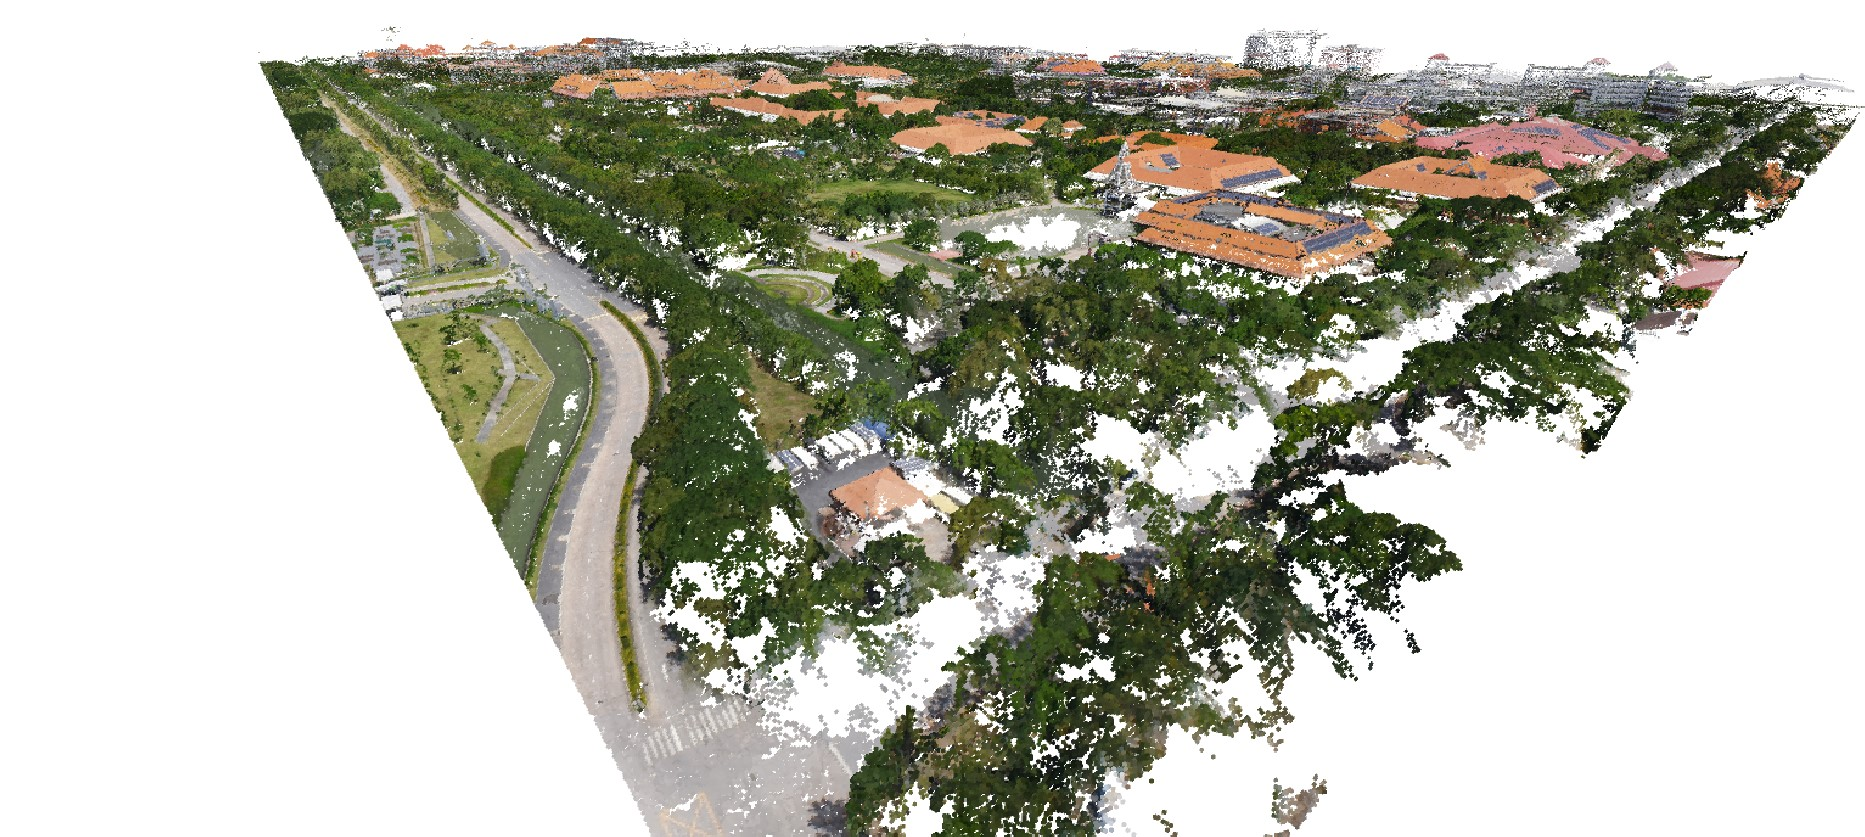
\includegraphics[width=\textwidth]{figs/results/lod-urban-800.jpg}
        \caption{LOD 800-1600-3200}
    \end{subfigure}
    
    \begin{subfigure}{0.9\textwidth}
        \centering
        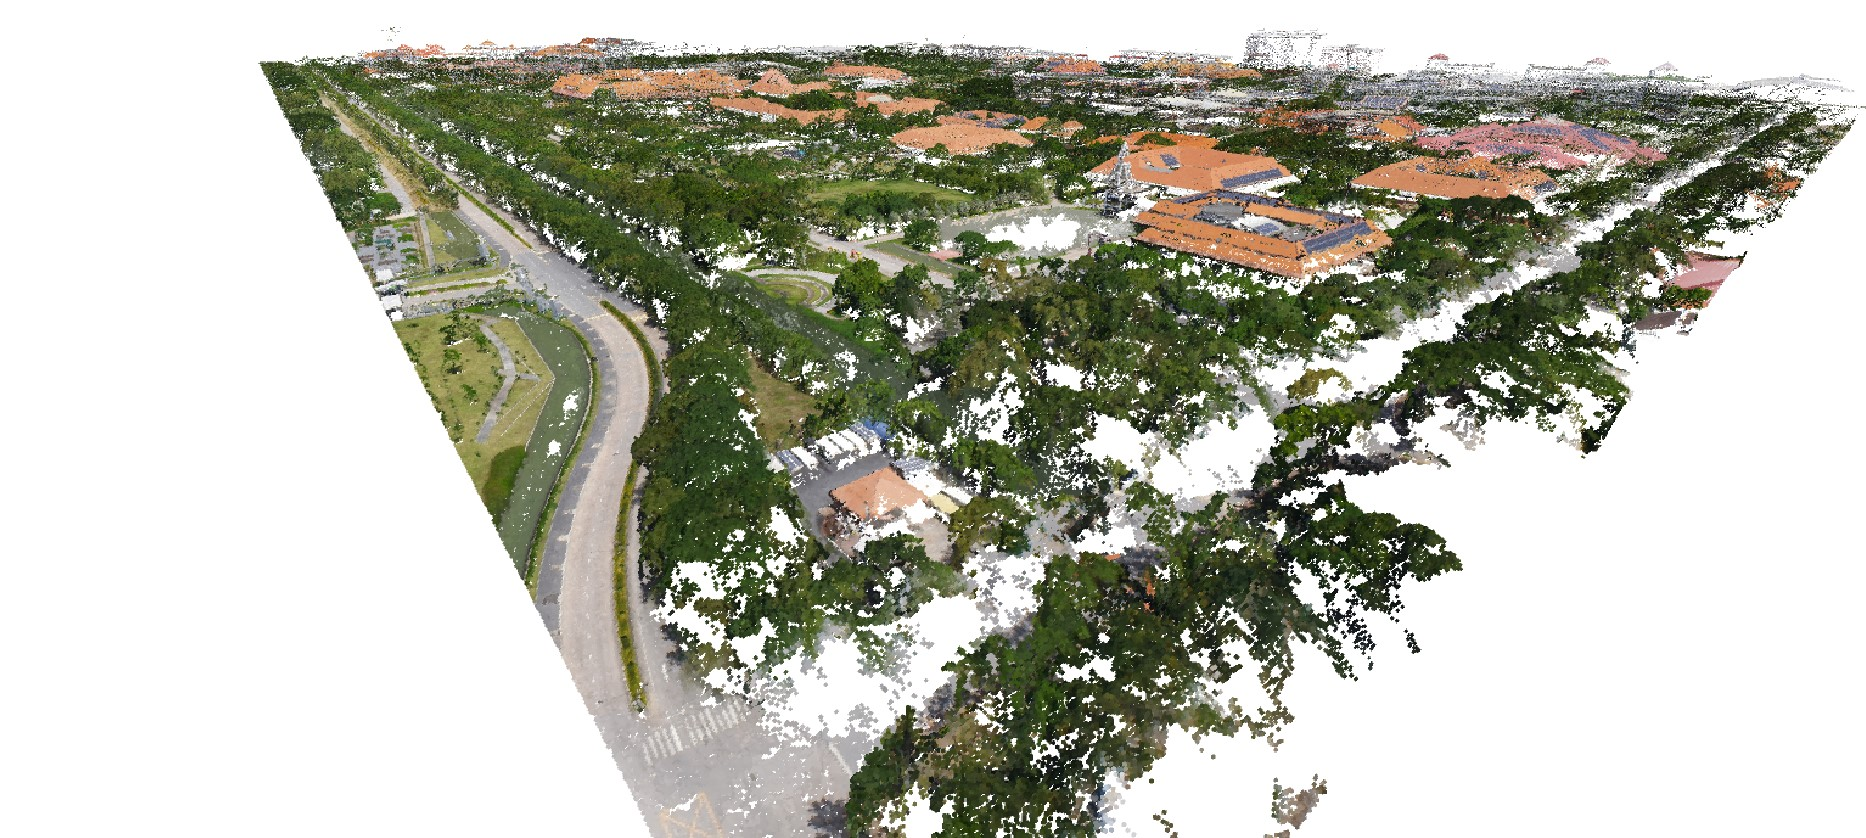
\includegraphics[width=\textwidth]{figs/results/lod-urban-400.jpg}
        \caption{LOD 400-800-1600}
    \end{subfigure}
    
    \begin{subfigure}{0.9\textwidth}
        \centering
        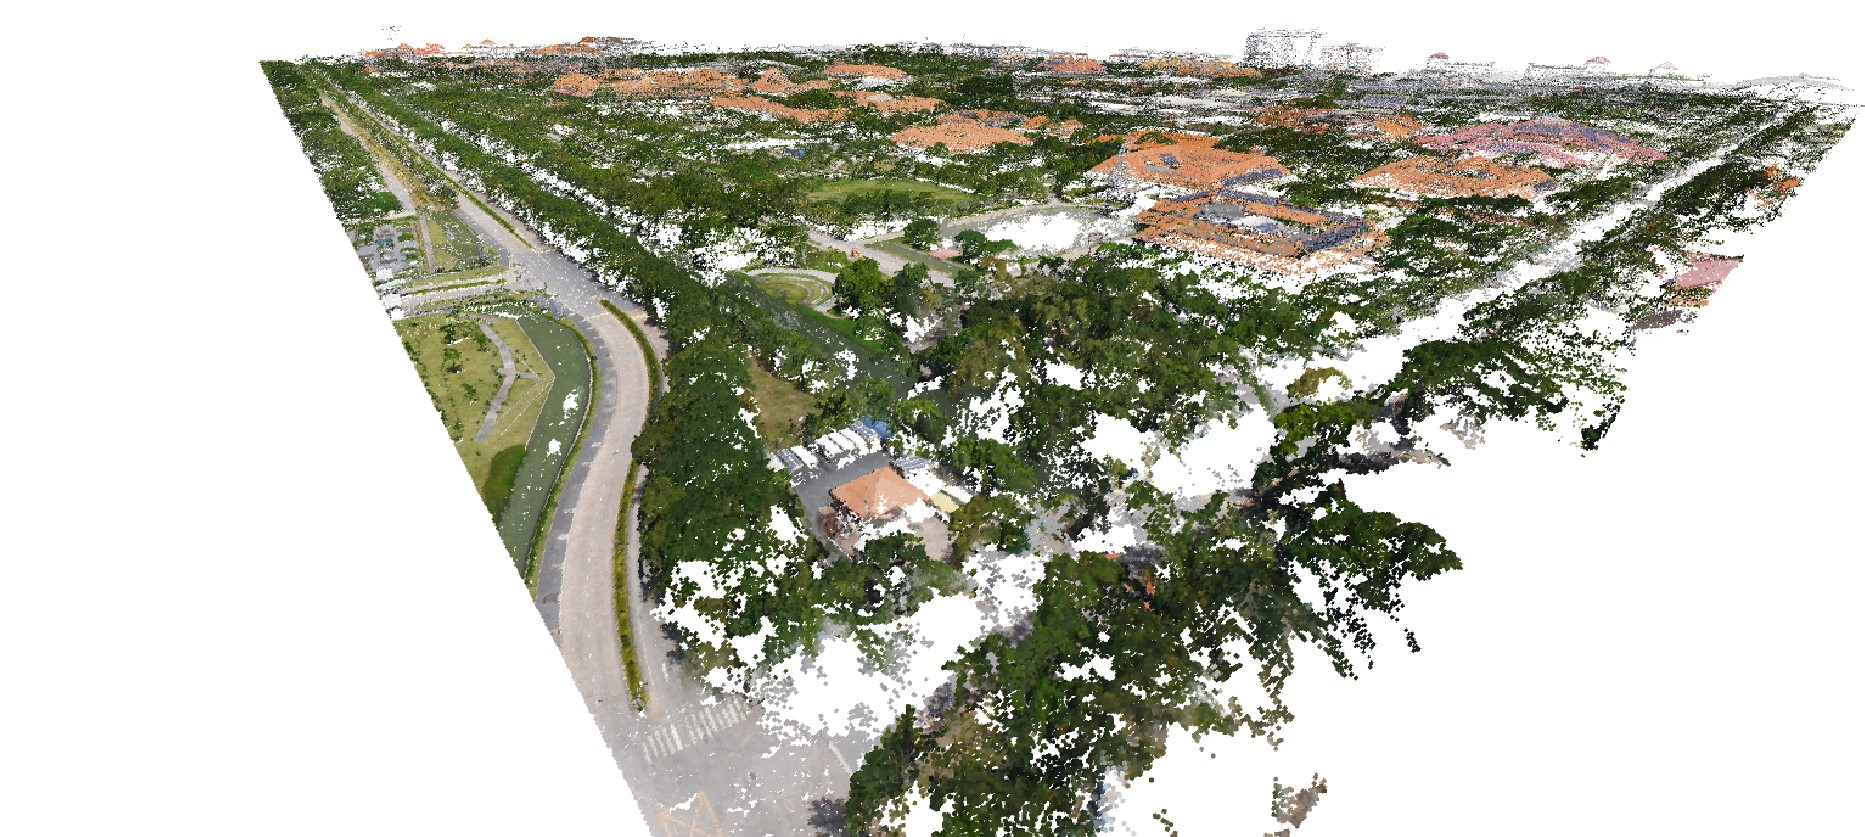
\includegraphics[width=\textwidth]{figs/results/lod-urban-200.jpg}
        \caption{LOD 200-800-1600}
    \end{subfigure}
    
    \caption{Urban scene rendered with LODs.}
\end{figure}

\begin{figure}[h]
    \centering
    
    \begin{subfigure}{0.7\textwidth}
        \centering
        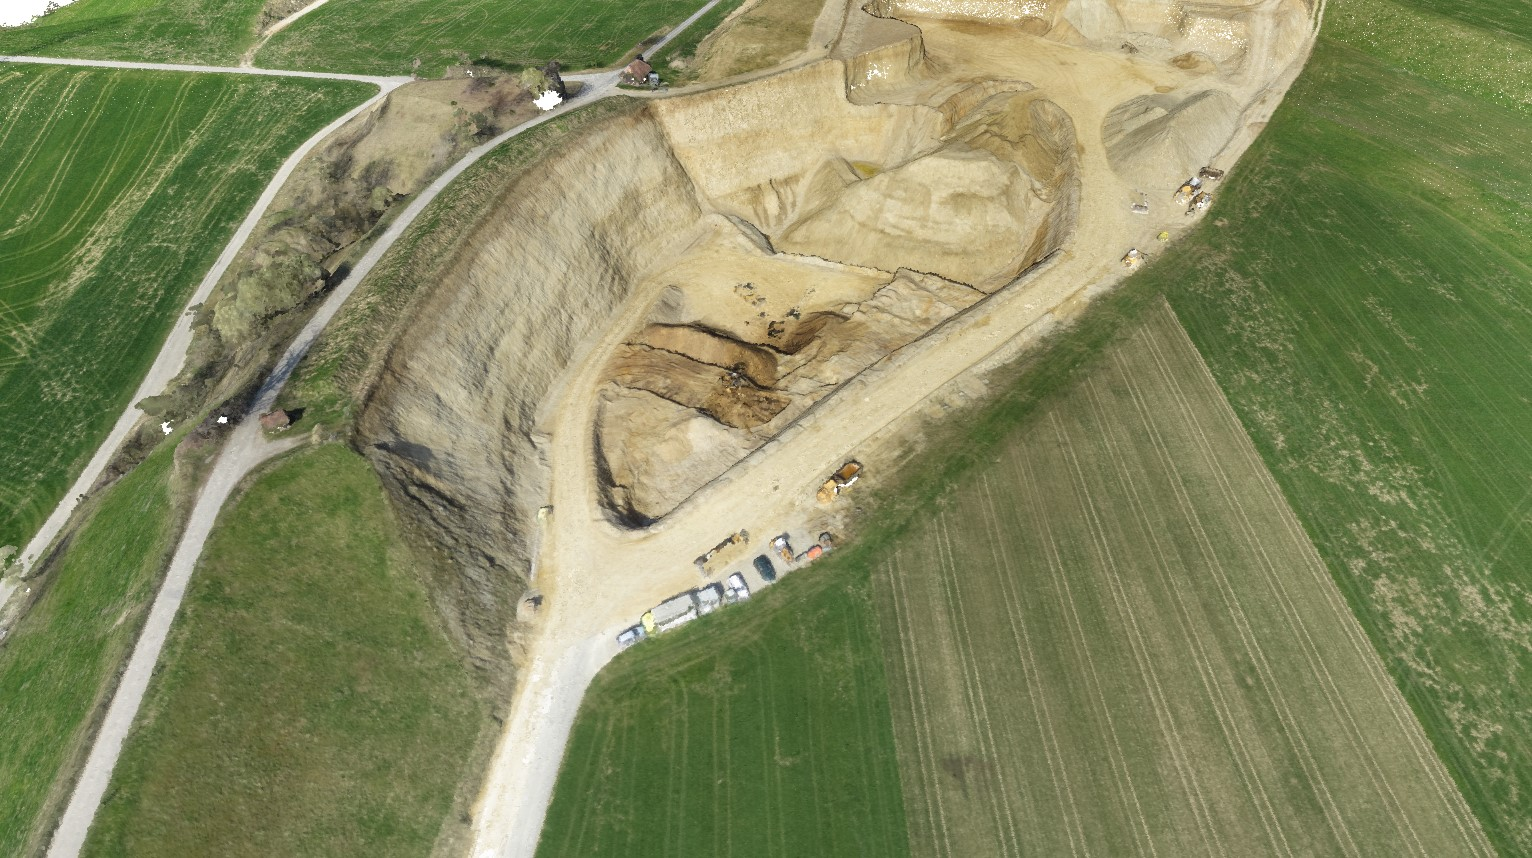
\includegraphics[width=\textwidth]{figs/results/lod-landscape-300.jpg}
        \caption{LOD 300-600-1200}
    \end{subfigure}
    
    \begin{subfigure}{0.7\textwidth}
        \centering
        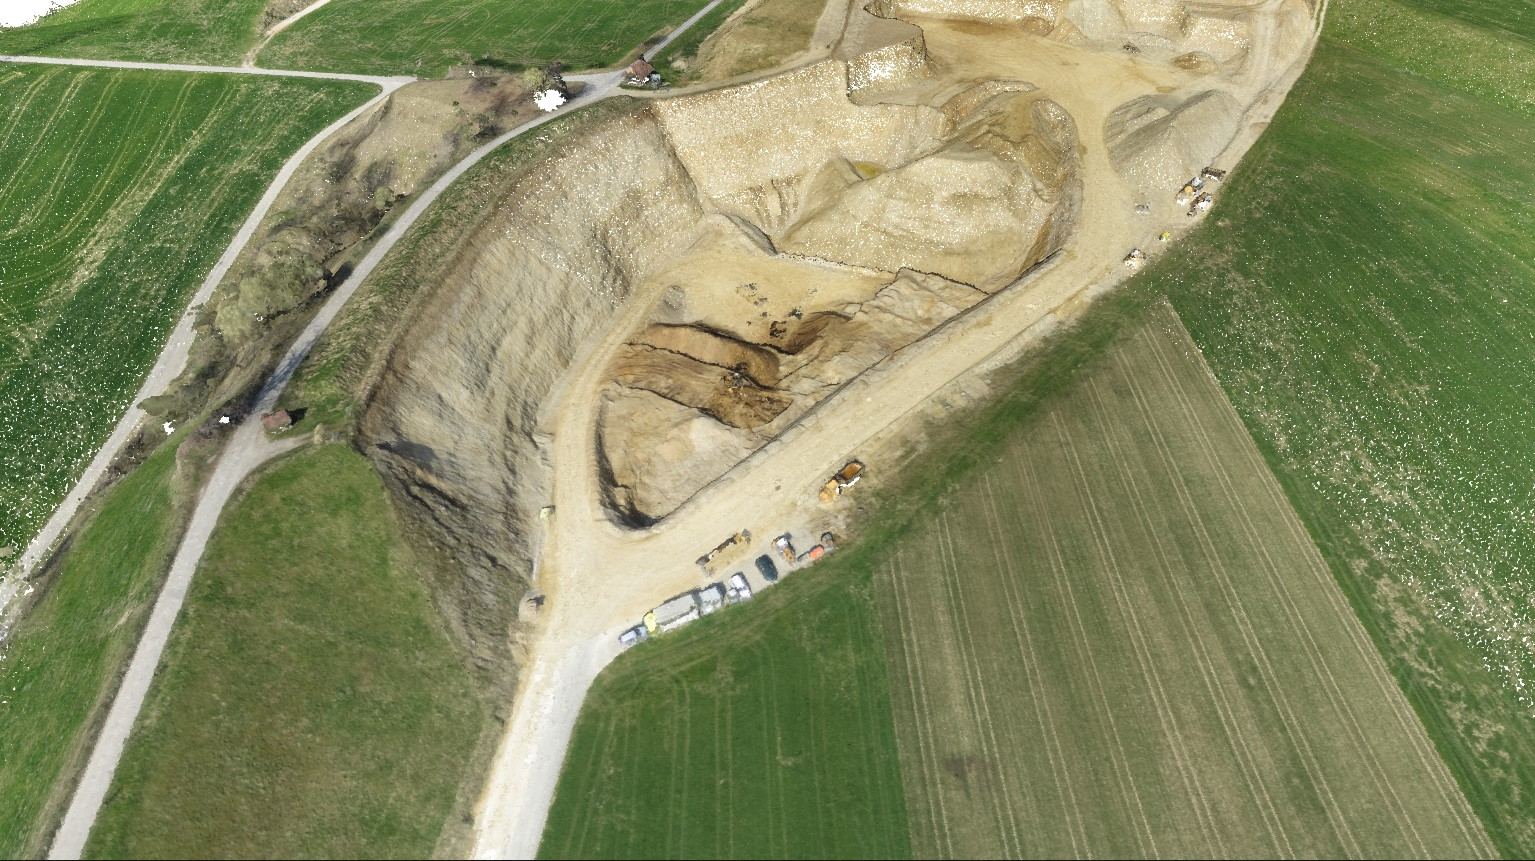
\includegraphics[width=\textwidth]{figs/results/lod-landscape-200.jpg}
        \caption{LOD 200-400-800}
    \end{subfigure}
    
    \begin{subfigure}{0.7\textwidth}
        \centering
        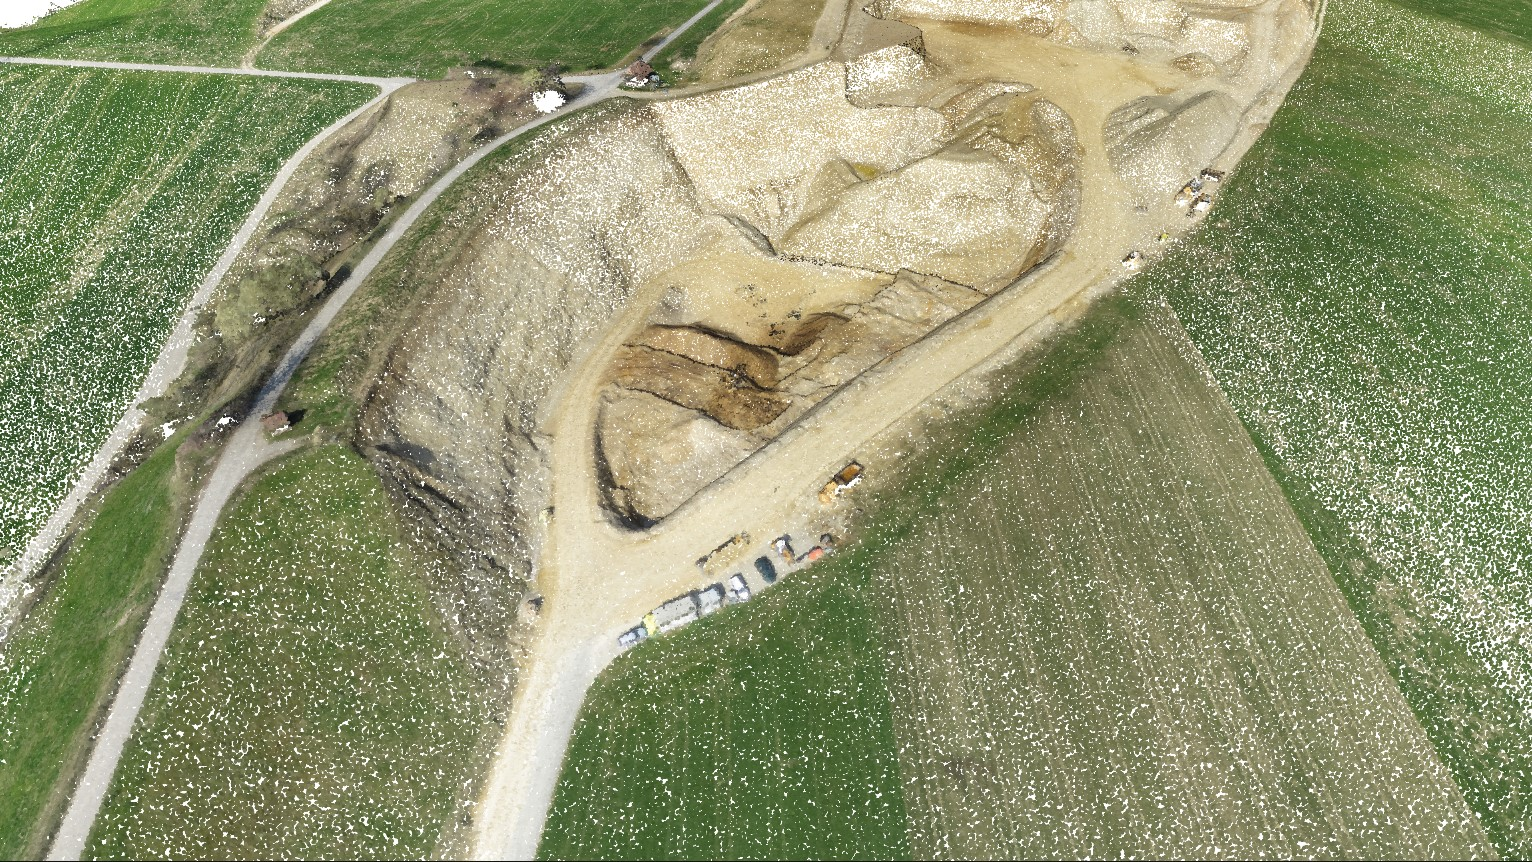
\includegraphics[width=\textwidth]{figs/results/lod-landscape-100.jpg}
        \caption{LOD 100-200-400}
    \end{subfigure}
    
    \caption{Landscape scene rendered with LODs.}
\end{figure}

\begin{figure}[h]
    \centering
    
    \begin{subfigure}{0.9\textwidth}
        \centering
        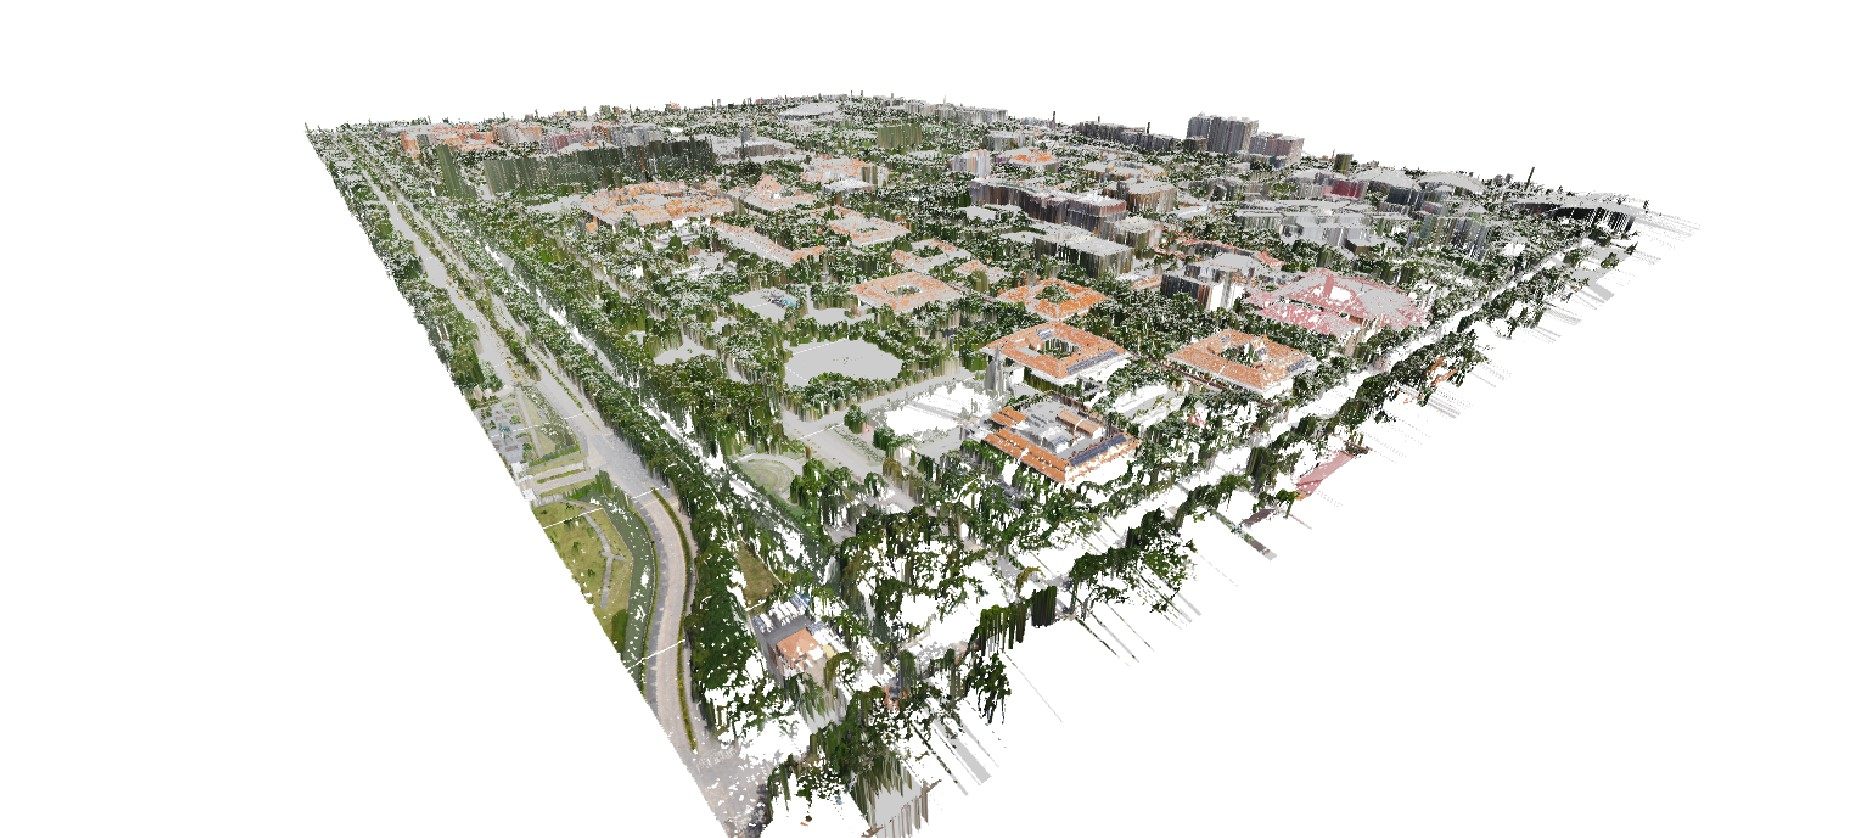
\includegraphics[width=\textwidth]{figs/results/mesh-urban-256.jpg}
        \caption{Mesh w. chunk resolution 256}
    \end{subfigure}
    
    \begin{subfigure}{0.9\textwidth}
        \centering
        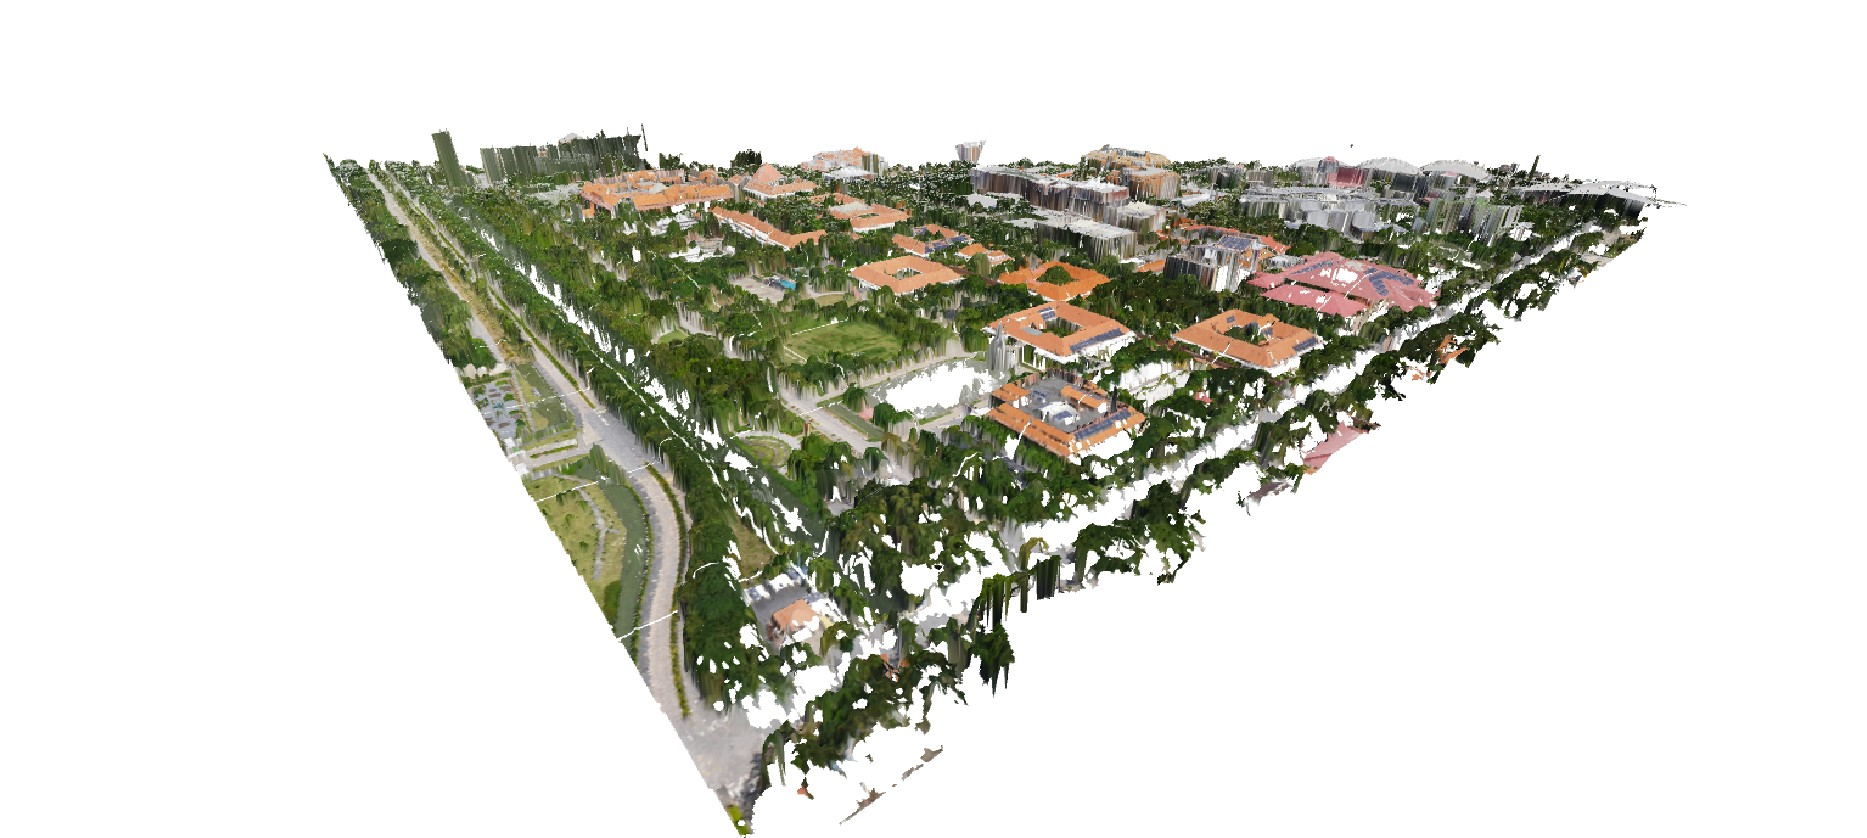
\includegraphics[width=\textwidth]{figs/results/mesh-urban-128.jpg}
        \caption{Mesh w. chunk resolution 128}
    \end{subfigure}
    
    \begin{subfigure}{0.9\textwidth}
        \centering
        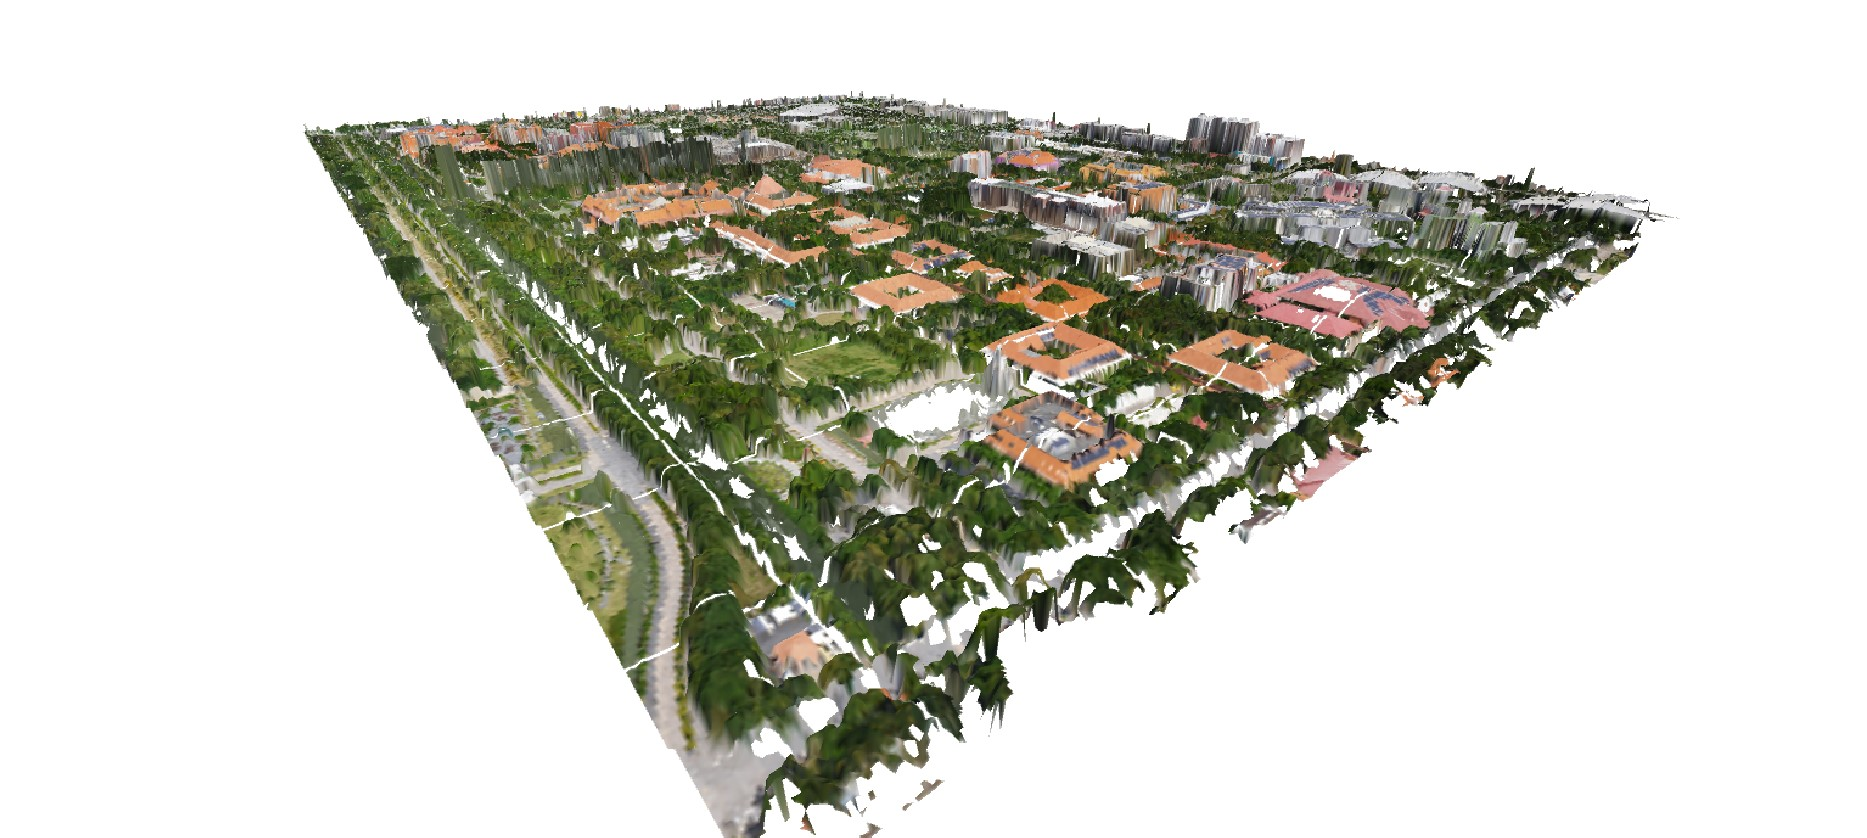
\includegraphics[width=\textwidth]{figs/results/mesh-urban-64.jpg}
        \caption{Mesh w. chunk resolution 64}
    \end{subfigure}
    
    \caption{Urban scene rendered with generated mesh.}
\end{figure}

\begin{figure}[h]
    \centering
    
    \begin{subfigure}{0.7\textwidth}
        \centering
        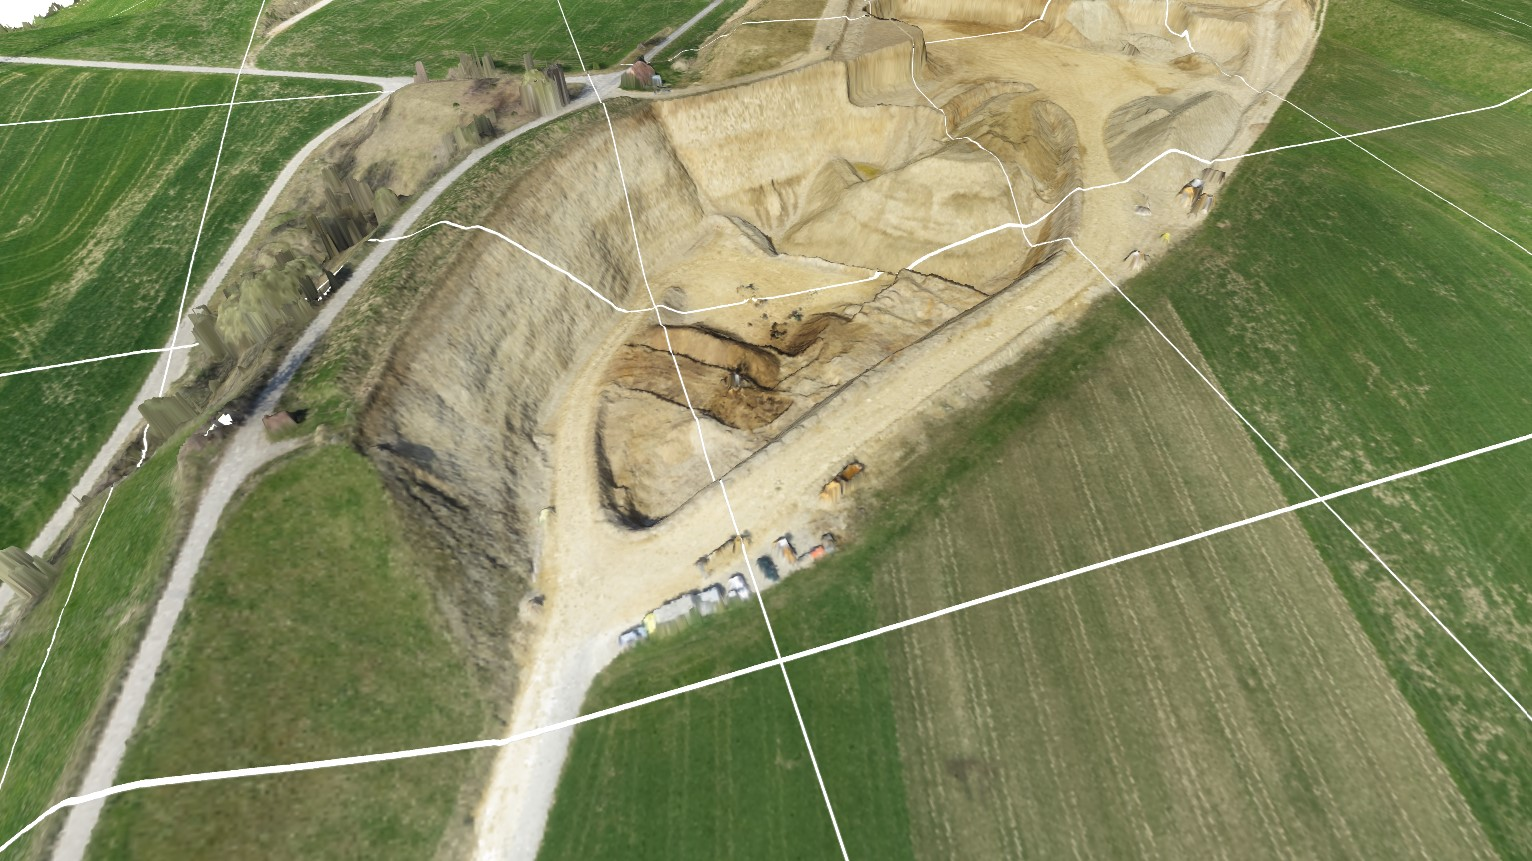
\includegraphics[width=\textwidth]{figs/results/mesh-landscape-256.jpg}
        \caption{Mesh w. chunk resolution 256}
    \end{subfigure}
    
    \begin{subfigure}{0.7\textwidth}
        \centering
        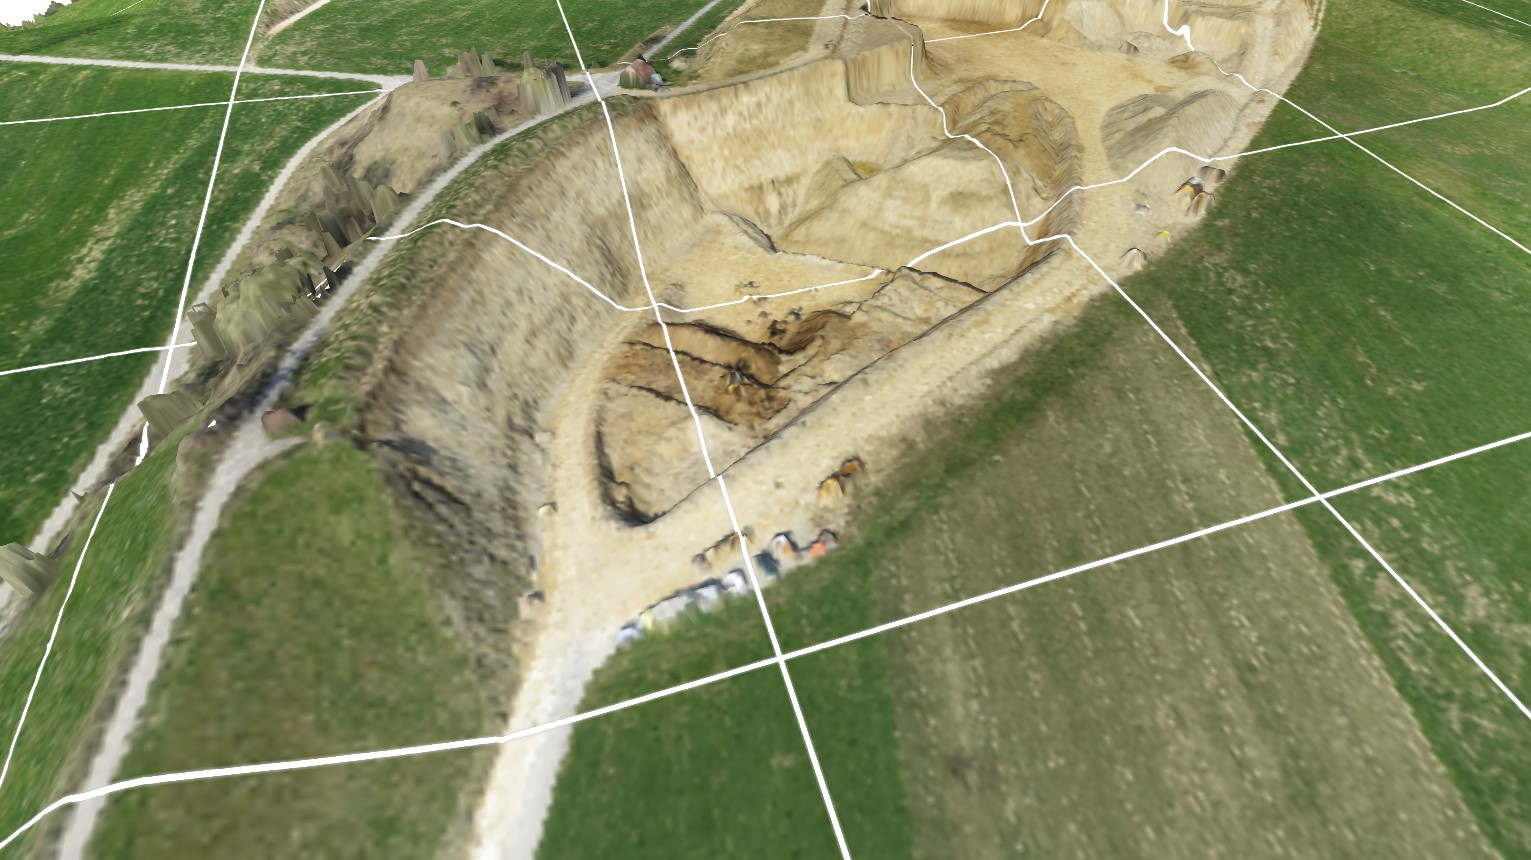
\includegraphics[width=\textwidth]{figs/results/mesh-landscape-128.jpg}
        \caption{Mesh w. chunk resolution 128}
    \end{subfigure}
    
    \begin{subfigure}{0.7\textwidth}
        \centering
        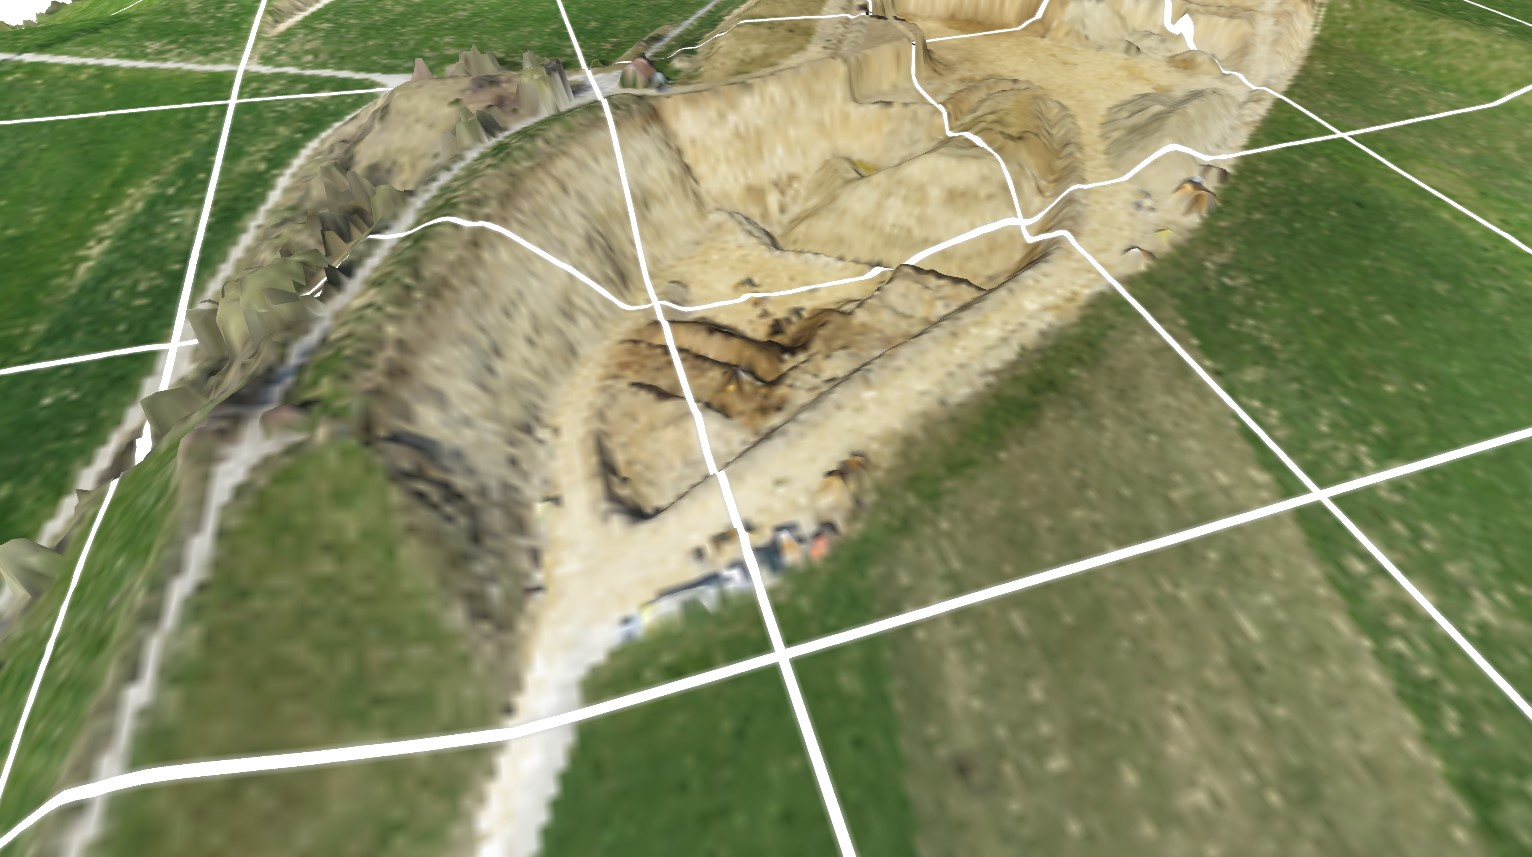
\includegraphics[width=\textwidth]{figs/results/mesh-landscape-64.jpg}
        \caption{Mesh w. chunk resolution 64}
    \end{subfigure}
    
    \caption{Landscape scene rendered with generated mesh.}
\end{figure}
